\documentclass{beamer}

\usepackage[utf8]{inputenc}
\usepackage[francais]{babel}
\usepackage{tikz}

\title{Recherche de chemin par dépôt de phéromones}
\author{Merwan Achibet}
\institute{Université du Havre}
\date{}

\usetheme{Warsaw}

\setbeamertemplate{navigation symbols}{}
\setbeamertemplate{footline}[frame number]

\definecolor{Backdrop}{RGB}{85, 98, 112}
\definecolor{Foreground}{RGB}{238, 238, 238}
\definecolor{Fabulous}{RGB}{210, 111, 127}

\usecolortheme[named=Backdrop]{structure}
\setbeamerfont{title}{series=\bfseries}
\setbeamercolor{title}{bg=Backdrop}
\setbeamercolor{frametitle}{fg=white, bg=Backdrop}
\setbeamercolor{normal text}{fg=Backdrop, bg=white}

\setbeamertemplate{blocks}[rounded][shadow=true]
\setbeamerfont{block title}{series=\bfseries}
\setbeamercolor{block title}{fg=white, bg=Backdrop!105}
\setbeamercolor{block body}{fg=Foreground, bg=Backdrop!80}

\setbeamertemplate{items}[circle]
\setbeamercolor{item}{fg=Fabulous!50}

\setbeamerfont{footline}{size=\small}

\begin{document}

\maketitle

\begin{frame}

  \frametitle{Sujet}

  \begin{block}{Le modèle}
    \begin{itemize}
    \item{Guidage de véhicules par phéromones synthétiques}
    \item{Parunak, Brueckner et Sauter (2002)}
    \end{itemize}
  \end{block}

  \vfill

  \begin{block}{L'implémentation}
    \begin{itemize}
    \item{En NetLogo}
    \item{José M. Vidal (2010)}
    \end{itemize}
  \end{block}

\end{frame}

\section{Le modèle}

\begin{frame}

  \frametitle{Analogie avec le vivant}

  \begin{block}{Les fourmis}
    \begin{itemize}
    \item{Fragiles, minuscules}
    \item{Une espèce pourtant prospère}
    \item{Grâce à son caractère social}
    \end{itemize}
  \end{block}

  \vfill

  \begin{block}{Coopération $\rightarrow$ communication}
    Par des signaux chimiques, les phéromones
    \begin{itemize}
      \item{Piste vers une source de nourriture}
      \item{Délimitation d'un territoire}
      \item{Zone dangereuse}
      \item{Disposition à la reproduction}
    \end{itemize}
  \end{block}

\end{frame}

\begin{frame}

  \frametitle{Analogie avec le vivant}

  Les phéromones sont soumises à différents phénomènes naturels :
  \begin{description}
    \item[\'Evaporation]{\'Ephémères, elles disparaissent progressivement}
    \item[Diffusion]{Volatiles, elles s'étalent}
  \end{description}

  \vfill

  \begin{block}{\'Emergence de pistes}
    \begin{itemize}
    \item{Les meilleures sont renforcées}
    \item{Les mauvaises s'effacent}
    \end{itemize}
  \end{block}

\end{frame}

\begin{frame}

  \frametitle{Adapté pour les systèmes multi-agents}

  Les phéromones rassemblent plusieurs qualités notables :

  \vfill

  \begin{block}{}
    \begin{description}[Décentralisation]
    \item[Diversité]{Une phéromone peut prendre n'importe quel sens}
    \item[Distribution]{Elles sont réparties sur l'environnement}
    \item[Décentralisation]{Une fourmi est un agent parmi d'autres}
    \item[Dynamicité]{S'adapte aux changements de l'environnement}
    \end{description}
  \end{block}

\end{frame}

\begin{frame}

  \frametitle{Le modèle de Parunak \textit{et al.}}

  \begin{block}{Utilisation de phéromones dans un cadre militaire}
    \begin{itemize}
    \item{Environnement  $\rightarrow$ zone de conflit divisée en blocs}
    \item{Fourmis $\rightarrow$ drones aériens}
    \item{Nourriture $\rightarrow$ bâtiments cibles}
    \item{Dangers $\rightarrow$ bâtiments menaces}
    \end{itemize}
  \end{block}

  \begin{figure}
    \centering
    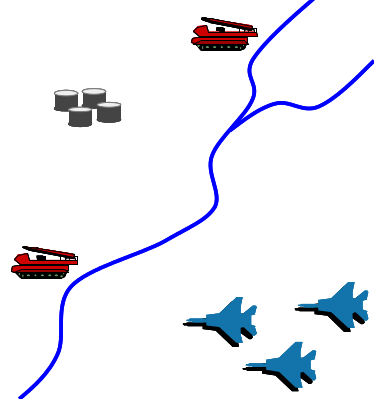
\includegraphics[width=3.5cm]{terrain_real.png}
  \end{figure}

\end{frame}

\begin{frame}

  \frametitle{Phéromones employées}

  \begin{block}{Par les drones}
    \begin{description}
    \item[GTarget]{Mène à une cible}
    \item[GNest]{Mène à la base}
    \end{description}
  \end{block}

  \begin{block}{Par les bâtiments}
    \begin{description}
    \item[RTarget]{Libérée par les cibles, elle \textit{attire}}
    \item[RThreat]{Libérée par les menaces, elle \textit{repousse}}
    \end{description}
  \end{block}

  \vfill

  \begin{figure}
    \centering
    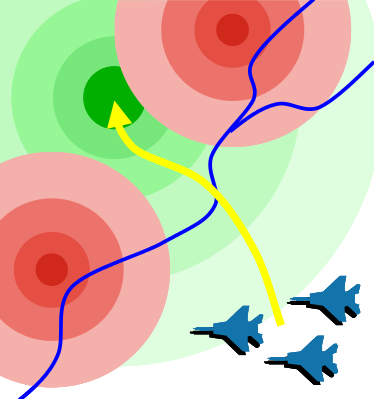
\includegraphics[width=3.2cm]{terrain_field.png}
  \end{figure}

\end{frame}

\begin{frame}

  \frametitle{Guidage}

  \begin{block}{Pour se diriger}
    \begin{itemize}
    \item{On ne veut pas évaluer chaque phéromone séparément}
    \item{On calcule une phéromone nette décrivant l'attractivité}
    \end{itemize}
  \end{block}

  \vfill

  $$g = \frac{ \theta \operatorname{RTarget} + \gamma \operatorname{GTarget} + \beta}{\alpha \operatorname{RThreat} + \delta \operatorname{Dist} + \beta}$$

\end{frame}


\begin{frame}

  \frametitle{Un nouveau type d'agent}

  \begin{block}{Les fantômes}
    \begin{itemize}
    \item{Courte durée de vie}
    \item{Haute vitesse}
    \end{itemize}
  \end{block}

  \vfill

  \begin{figure}
    \centering
    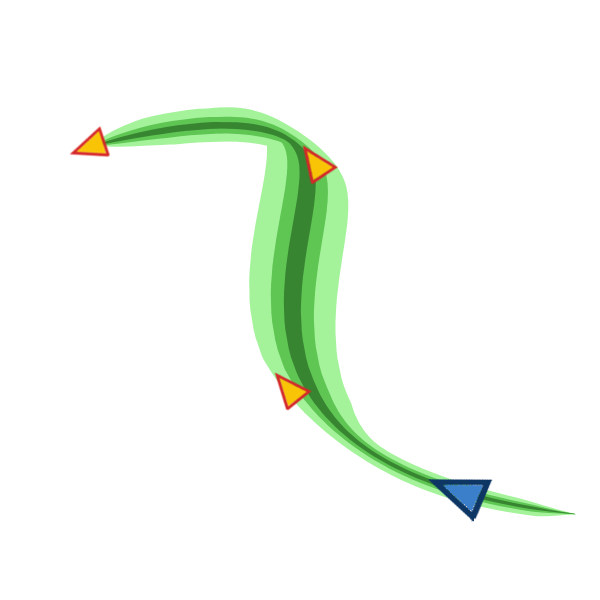
\includegraphics[width=4cm]{ghosts.png}
  \end{figure}

  \vfill

  Ils permettent d'évaluer les chemins que le drone pourrait arpenter
  dans un futur proche.

\end{frame}

\section{L'implémentation}

\begin{frame}

  \frametitle{L'implémentation de José M. Vidal}

  \begin{block}{}
    \begin{itemize}
    \item{Zones $\rightarrow$ \textit{patches}}
    \item{Agents (drones, fantomes, bâtiments) $\rightarrow$ \textit{turtles}}
    \end{itemize}
  \end{block}

  \vfill

  \begin{block}{La simulation}
    \begin{itemize}
    \item{Environnement aléatoirement généré}
    \item{Un unique drone}
    \item{Objectif : atteindre une cible}
    \item{On ne se soucie pas du retour à la base}
    \end{itemize}
  \end{block}

\end{frame}

\begin{frame}

  \begin{figure}
    \centering
    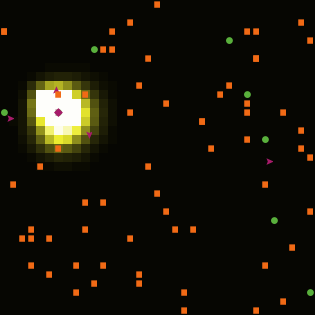
\includegraphics[width=7cm]{pheromones_tohome.png}
  \end{figure}

  \vfill

  \begin{center}
    GNest
  \end{center}

\end{frame}

\begin{frame}

  \begin{figure}
    \centering
    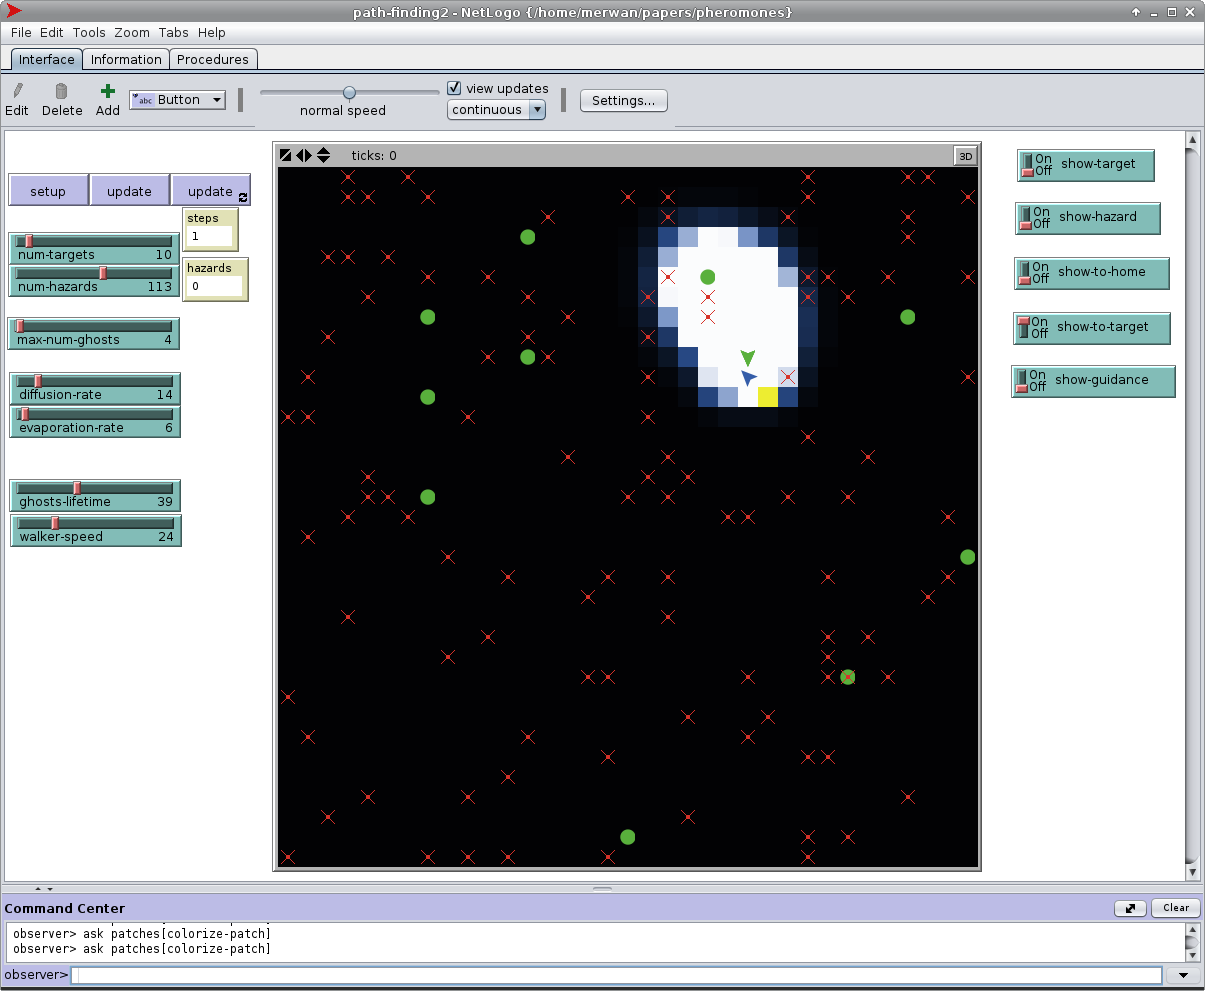
\includegraphics[width=7cm]{pheromones_totarget.png}
  \end{figure}

  \vfill

  \begin{center}
    GTarget
  \end{center}

\end{frame}

\begin{frame}

  \begin{figure}
    \centering
    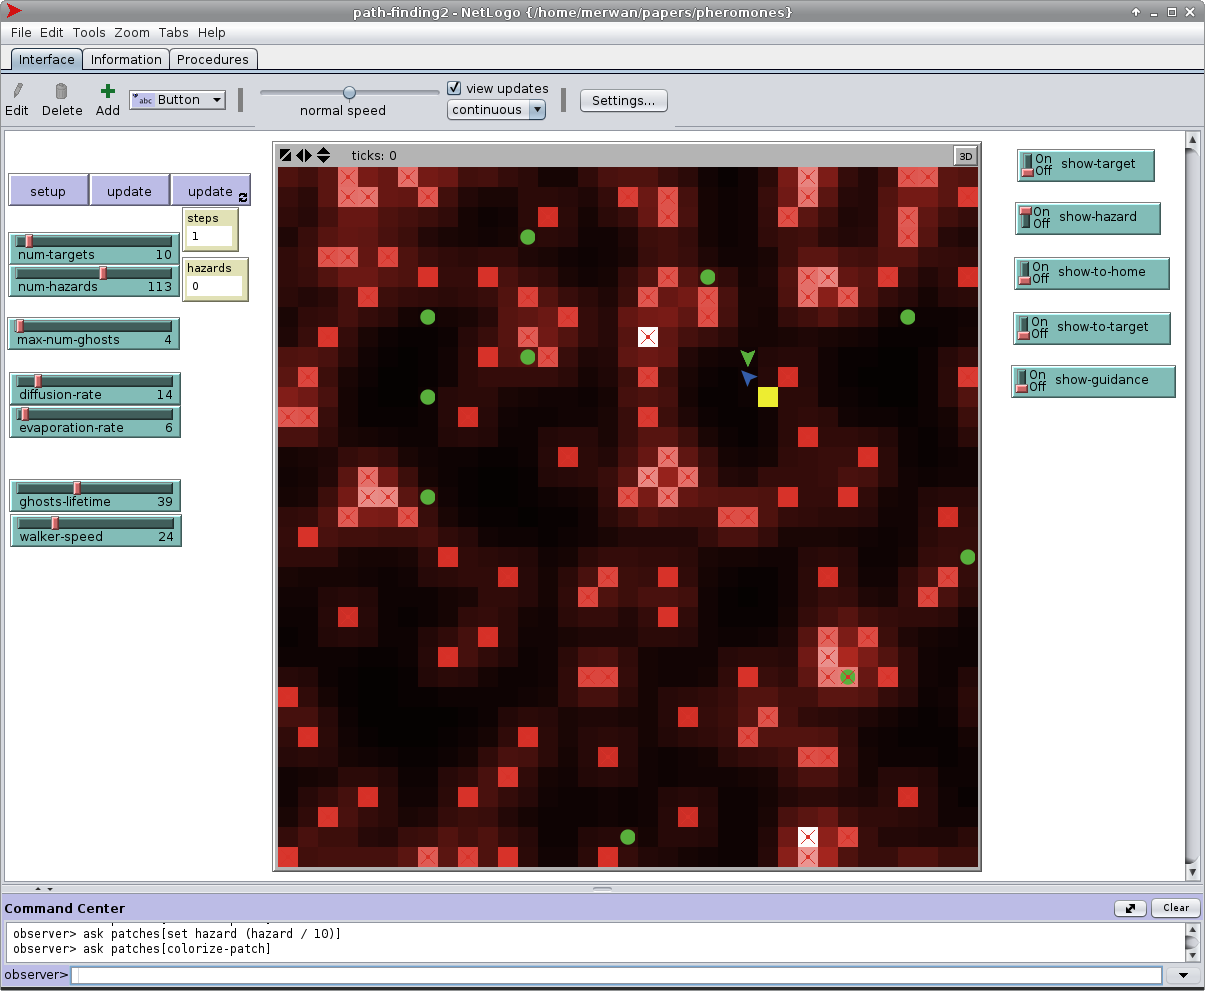
\includegraphics[width=7cm]{pheromones_hazard.png}
  \end{figure}

  \vfill

  \begin{center}
    RThreat
  \end{center}

\end{frame}

\begin{frame}

  \begin{figure}
    \centering
    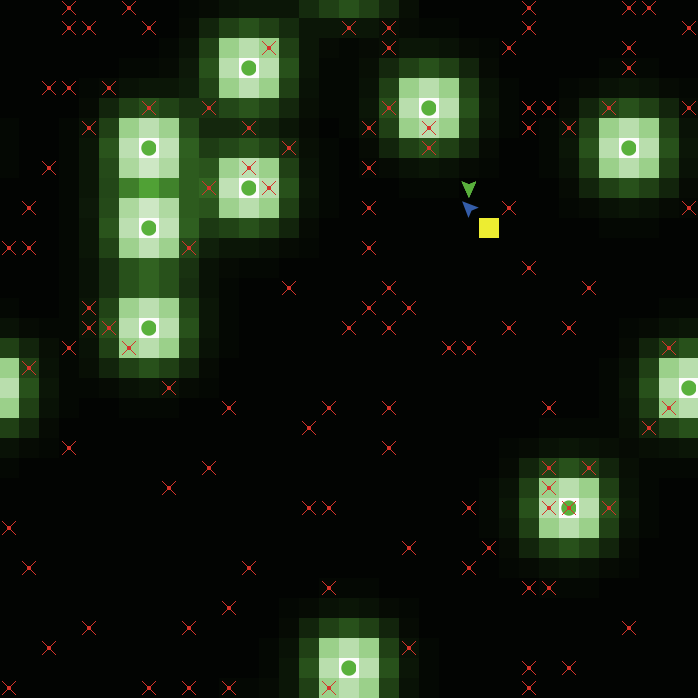
\includegraphics[width=7cm]{pheromones_target.png}
  \end{figure}

  \vfill

  \begin{center}
    RTarget
  \end{center}

\end{frame}

\begin{frame}

  \frametitle{Problème : un guidage trop simpliste}

  \begin{block}{Dans le code}
    \begin{itemize}
    \item{\texttt{uphill RTarget} guide les fantômes}
    \item{\texttt{uphill GTarget} guide le drone}
    \end{itemize}
  \end{block}

  \vfill

  La fonction d'évaluation de l'attractivité n'est pas utilisée
  \begin{itemize}
    \item{Le drone suit toujours le chemin le plus court...}
    \item{... Mais ignore les dangers !}
  \end{itemize}

\end{frame}

\begin{frame}

  \begin{figure}
    \centering
    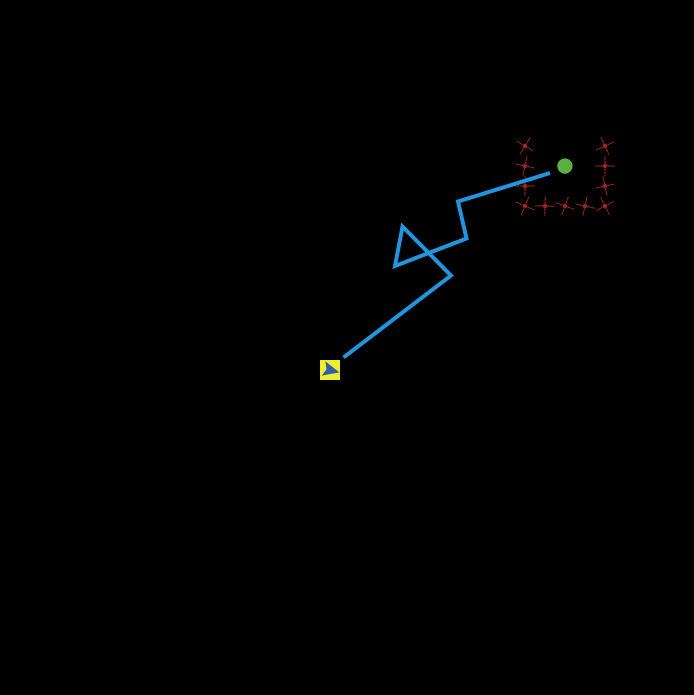
\includegraphics[width=7cm]{path1.png}
  \end{figure}

  \vfill

  \begin{center}
    Scénario critique
  \end{center}

\end{frame}

\begin{frame}

  \frametitle{Nouvelle version}

  L'attractivité de chaque case est mise à jour après chaque itération
  via la fonction $g$.

  \vfill

  \begin{block}{\'Etapes du déplacement d'un drone/fantôme}
    \begin{enumerate}
    \item{Observer l'attractivité des huits zones voisines}
    \item{Tirage aléatoire sur une roue de la fortune biaisée}
    \item{Déplacement sur la case gagnante}
    \end{enumerate}
  \end{block}

\end{frame}

\begin{frame}

  \begin{figure}
    \centering
    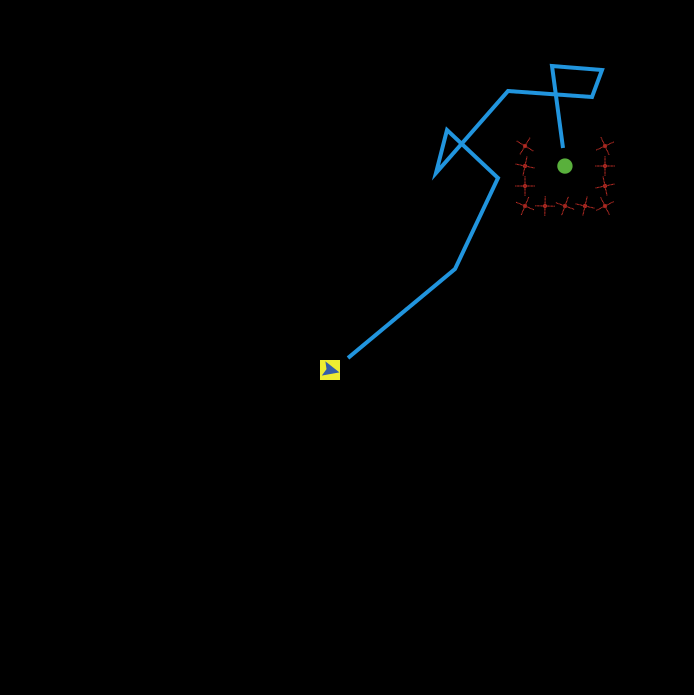
\includegraphics[width=7cm]{path2.png}
  \end{figure}

  \vfill

  \begin{center}
    Scénario critique
  \end{center}

\end{frame}

\begin{frame}

  \frametitle{Influence des réglages utilisateur}

  \begin{block}{Nombre de fantômes}
    \begin{description}
      \item[Trop faible]{Peu d'émergence}
    \end{description}
  \end{block}

  \vfill

  \begin{figure}
    \centering
    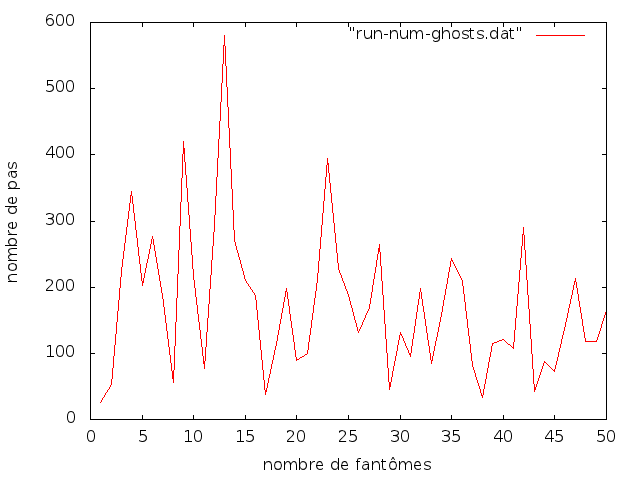
\includegraphics[width=7.2cm]{run-num-ghosts.png}
  \end{figure}

\end{frame}

\begin{frame}

  \frametitle{Influence des réglages utilisateur}

  \begin{block}{Taux de diffusion}
    \begin{description}
      \item[Trop faible]{Pistes étroites}
      \item[Trop élevé]{L'environnement est inondé}
    \end{description}
  \end{block}

  \vfill

  \begin{figure}
    \centering
    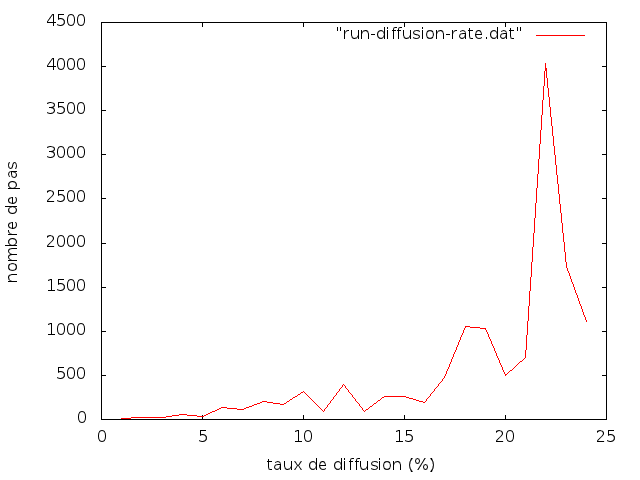
\includegraphics[width=7.2cm]{run-diffusion-rate.png}
  \end{figure}

\end{frame}

\begin{frame}

  \frametitle{Influence des réglages utilisateur}

  \begin{block}{Taux d'évaporation}
    \begin{description}
      \item[Trop faible]{Les mauvaises pistes perdurent et induisent
        en erreur}
      \item[Trop élevé]{Pas le temps de les suivre}
    \end{description}
  \end{block}

  \vfill

  \begin{figure}
    \centering
    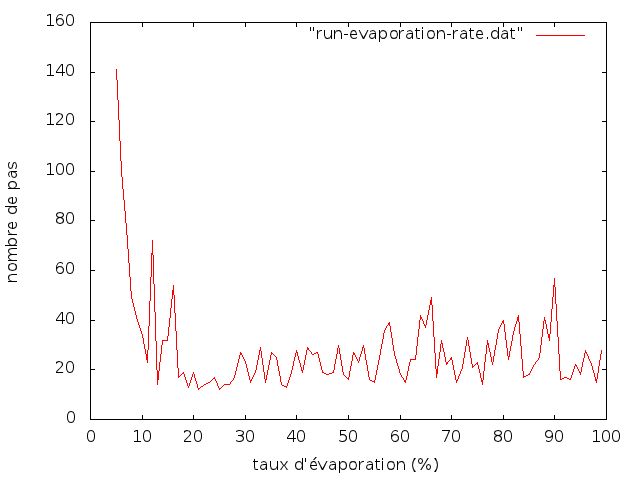
\includegraphics[width=7.2cm]{run-evaporation-rate.png}
  \end{figure}

\end{frame}

\begin{frame}

  \frametitle{Influence des facteurs de $g$}

  $$g = \frac{ \theta \operatorname{RTarget} + \gamma \operatorname{GTarget} + \beta}{\alpha \operatorname{RThreat} + \delta \operatorname{Dist} + \beta}$$

  \vfill

  \begin{block}{$\theta$ et $\gamma$}
    \begin{itemize}
    \item{$\theta \rightarrow$ importance des phéromones des
      bâtiments}
    \item{$\gamma \rightarrow$ importance des phéromones des
      fantômes}
    \item{$\theta < \gamma$, on \textit{fait confiance} aux
      fantômes}
    \end{itemize}
  \end{block}

  \vfill

  \begin{block}{$\alpha$}
    \begin{description}
    \item[Trop faible]{Risque de rencontrer un danger}
    \item[Trop élevé]{Configurations infranchissables}
    \end{description}
  \end{block}

\end{frame}

\end{document}
